\section{Results}

	\begin{center}
	\begin{tabular}{ l | c | r }
		\hline
		Parameters & Values $A, B$ & Description \\ \hline
		L & $7.5$ & Length half size demain  \\ 
		R & ? &  radius \\
	
		$\mu$ & 1  & ..\\
		$\nu_c$  & .&  . \\
		$\nu_d$  & .&  . \\
		k & . & .\\
		D & & \\
		$\beta$ & & \\
		$\delta$ & & \\
		%	$N_A$ & 250 & particles of type A\\
%	$N_B$ & 250 & particles of type B \\
		\hline
	\end{tabular}
\end{center}	




%----------PLOTS
% \begin{tabular}{cl}  
%	\begin{tabular}{c}
%		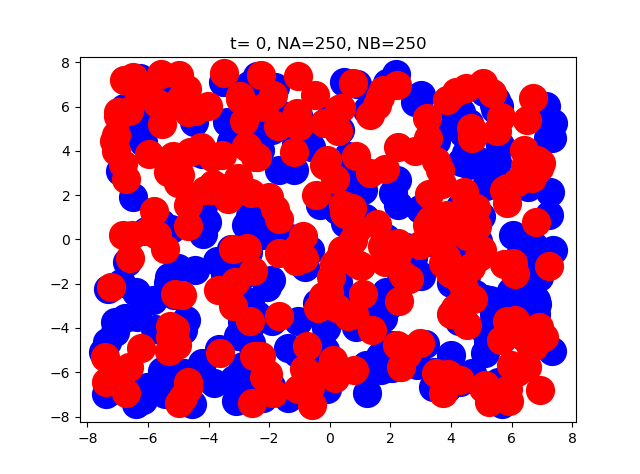
\includegraphics[height=4cm, width=4cm]{micro_ini_caseI1}
%	\end{tabular}
%	& \begin{tabular}{l}
%		\parbox{-0.2\linewidth}{%  change the parbox width as appropiate
%			%\textbf{text on equation}   
%			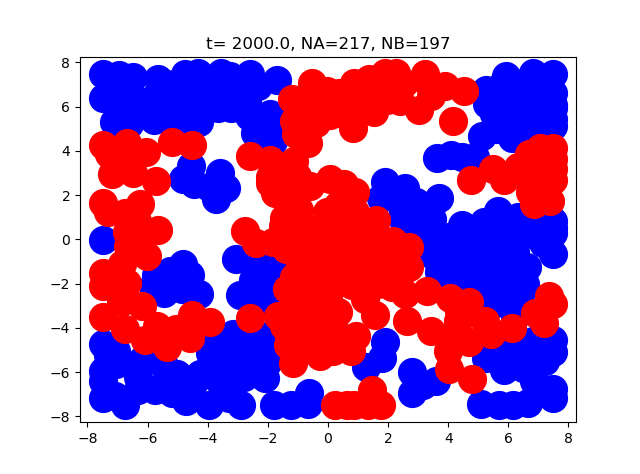
\includegraphics[height=4cm, width=4cm]{micro_fin_caseI1}
%			
%		}
%	\end{tabular}  \\
%\end{tabular}


% DO NOT DELETE - NE PAS EFFACHER
%	\begin{minipage}[h]{%0.5\linewidth}
%	\centering
%	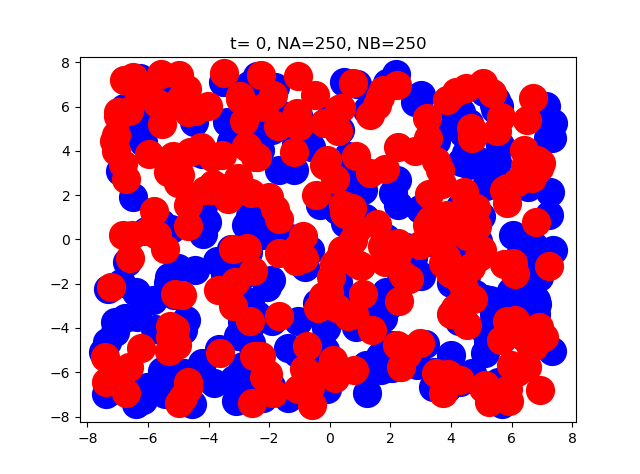
\includegraphics[width=1\linewidth]{micro_ini_caseI1}
%	%\captionof{figure}{ }\label{fig:1}
%	\end{minipage}
%\hfill
%	\begin{minipage}[h]{%0.5\linewidth}
%	\centering
%	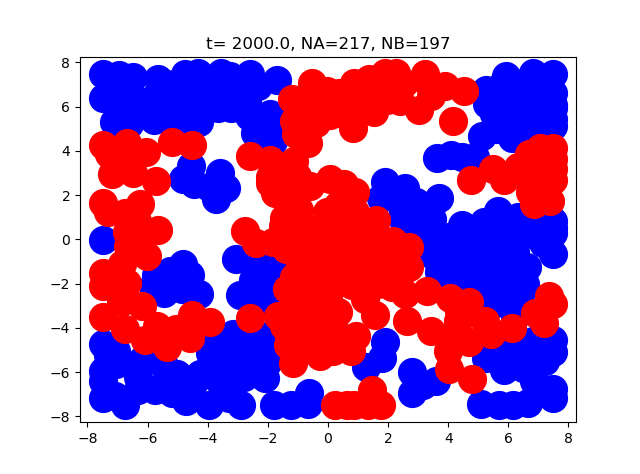
\includegraphics[width=1\linewidth]{micro_fin_caseI1}
%	%\captionof{figure}{ }\label{fig:2}
%	
%%{case I: A-cells blue, B-cells red with $k^{AA}=k^{BB}=2 $, $k^{AB}=k^{BA}=8$; $b0_A=b0_B=10^{-3}$, $d0_A=d0_B=7\cdot10^{-4}$}	
%	\end{minipage}
%-----------------------------------------------------

% DO NOT DELETE - NE PAS EFFACHER
%{case I: A-cells blue, B-cells red with $k^{AA}=k^{BB}=2 $, $k^{AB}=k^{BA}=8$; $b0_A=b0_B=2\cdot10^{-3}$, $d0_A=d0_B=7\cdot10^{-4}$}

%{case I: A-cells blue, B-cells red with $k^{AA}=k^{BB}=2 $, $k^{AB}=k^{BA}=8$; $b0_A=b0_B=10^{-4}$, $d0_A=d0_B=7\cdot10^{-5}, \th_A=\th_B=8\cdot 10^{-5}$}

%{case I: A-cells blue, B-cells red with $k^{AA}=k^{BB}=2 $, $k^{AB}=k^{BA}=4$; $b0_A=b0_B=10^{-4}$, $d0_A=d0_B=7\cdot10^{-5}, \th_A=\th_B=8\cdot 10^{-5}$}





